% Created by tikzDevice version 0.12.4 on 2023-10-26 11:29:03
% !TEX encoding = UTF-8 Unicode
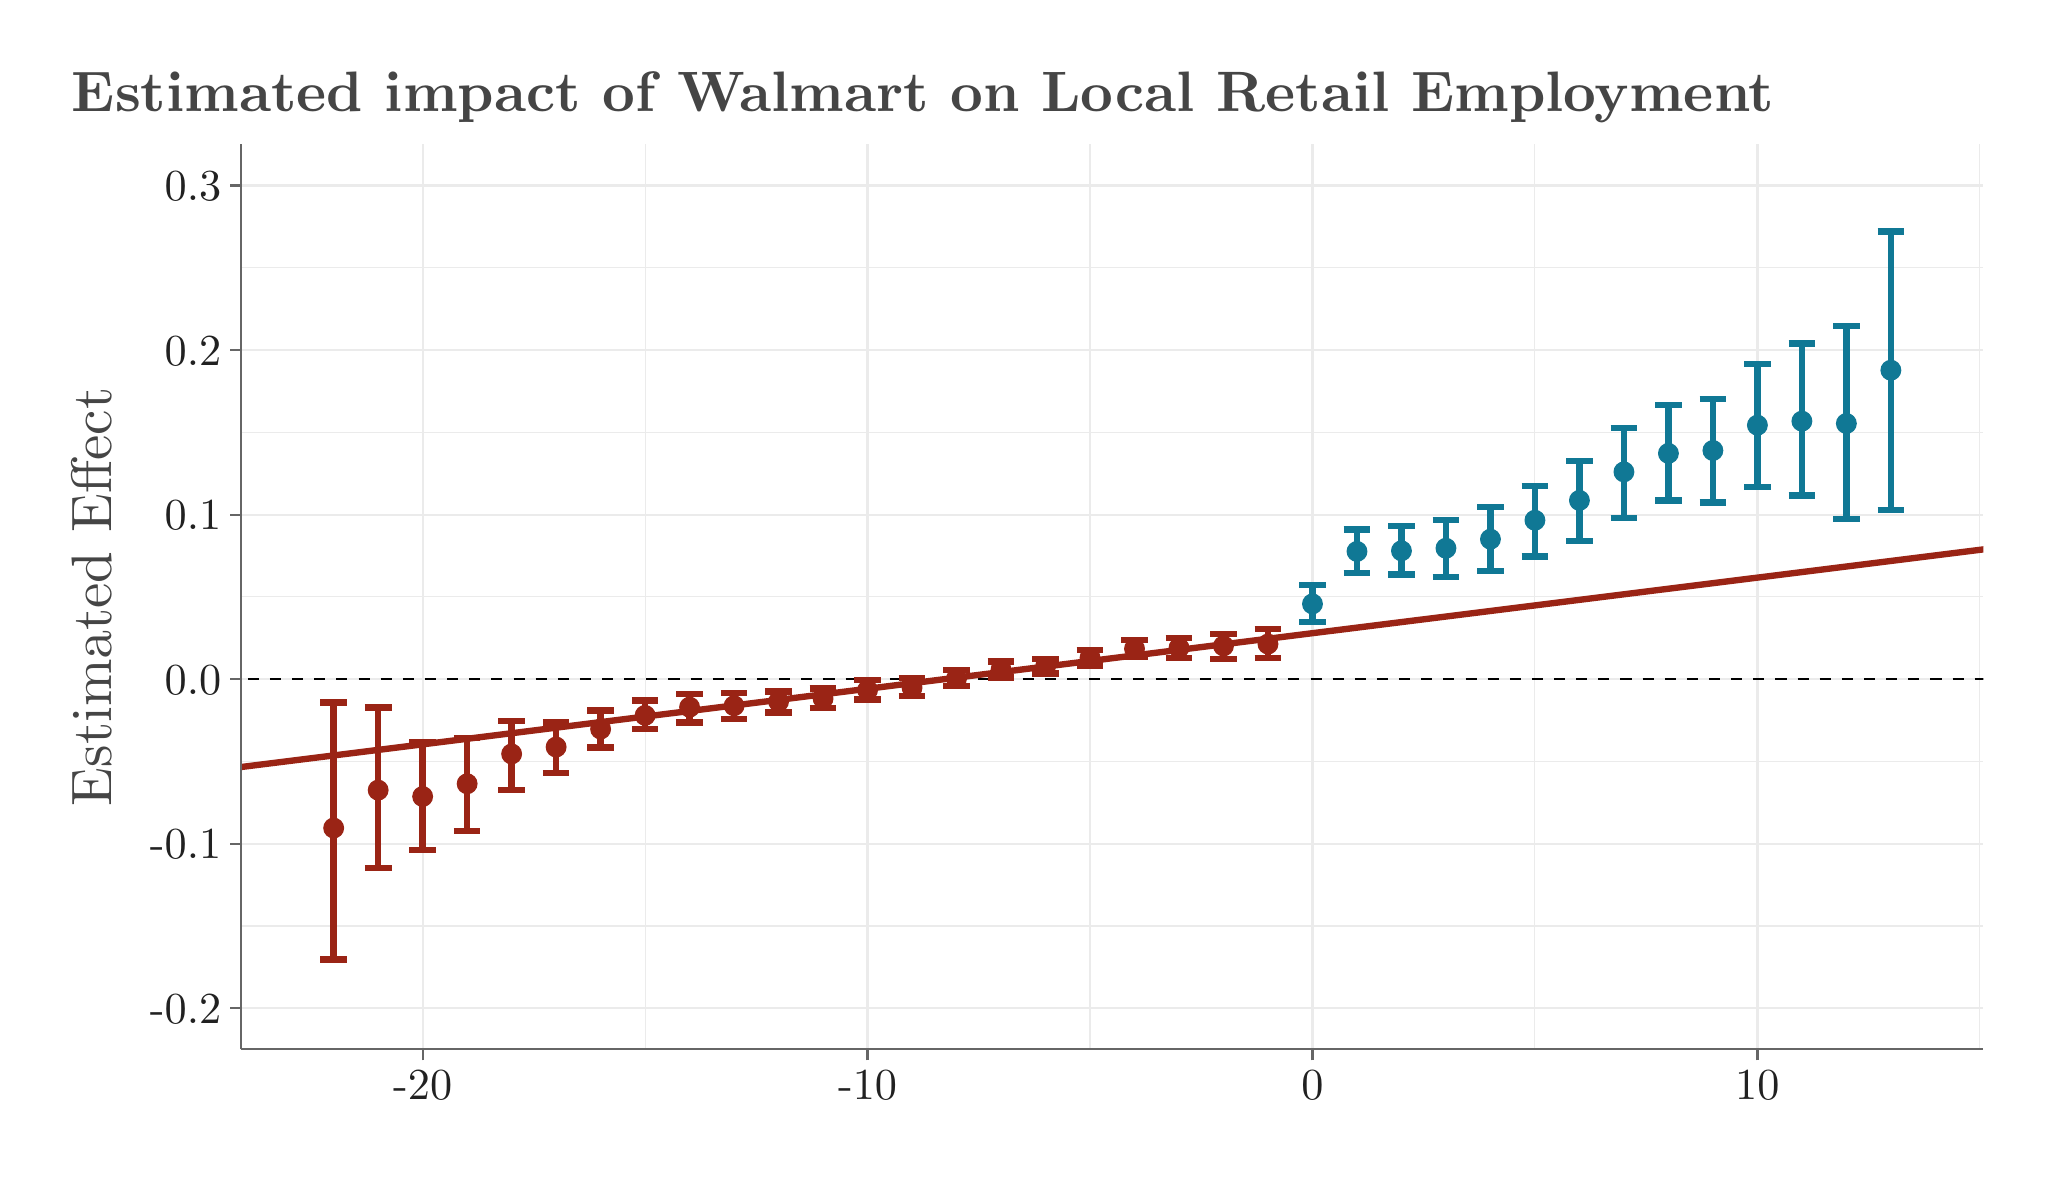
\begin{tikzpicture}[x=1pt,y=1pt]
\definecolor{fillColor}{RGB}{255,255,255}
\path[use as bounding box,fill=fillColor,fill opacity=0.00] (0,0) rectangle (722.70,406.52);
\begin{scope}
\path[clip] (  0.00,  0.00) rectangle (722.70,406.52);
\definecolor{fillColor}{RGB}{255,255,255}

\path[fill=fillColor] ( -0.00,  0.00) rectangle (722.70,406.52);
\end{scope}
\begin{scope}
\path[clip] ( 77.13, 37.33) rectangle (706.70,364.33);
\definecolor{fillColor}{RGB}{255,255,255}

\path[fill=fillColor] ( 77.13, 37.33) rectangle (706.70,364.33);
\definecolor{drawColor}{gray}{0.92}

\path[draw=drawColor,line width= 0.4pt,line join=round] ( 77.13, 81.92) --
	(706.70, 81.92);

\path[draw=drawColor,line width= 0.4pt,line join=round] ( 77.13,141.38) --
	(706.70,141.38);

\path[draw=drawColor,line width= 0.4pt,line join=round] ( 77.13,200.83) --
	(706.70,200.83);

\path[draw=drawColor,line width= 0.4pt,line join=round] ( 77.13,260.29) --
	(706.70,260.29);

\path[draw=drawColor,line width= 0.4pt,line join=round] ( 77.13,319.74) --
	(706.70,319.74);

\path[draw=drawColor,line width= 0.4pt,line join=round] (223.11, 37.33) --
	(223.11,364.33);

\path[draw=drawColor,line width= 0.4pt,line join=round] (383.88, 37.33) --
	(383.88,364.33);

\path[draw=drawColor,line width= 0.4pt,line join=round] (544.64, 37.33) --
	(544.64,364.33);

\path[draw=drawColor,line width= 0.4pt,line join=round] (705.41, 37.33) --
	(705.41,364.33);

\path[draw=drawColor,line width= 0.8pt,line join=round] ( 77.13, 52.19) --
	(706.70, 52.19);

\path[draw=drawColor,line width= 0.8pt,line join=round] ( 77.13,111.65) --
	(706.70,111.65);

\path[draw=drawColor,line width= 0.8pt,line join=round] ( 77.13,171.10) --
	(706.70,171.10);

\path[draw=drawColor,line width= 0.8pt,line join=round] ( 77.13,230.56) --
	(706.70,230.56);

\path[draw=drawColor,line width= 0.8pt,line join=round] ( 77.13,290.01) --
	(706.70,290.01);

\path[draw=drawColor,line width= 0.8pt,line join=round] ( 77.13,349.47) --
	(706.70,349.47);

\path[draw=drawColor,line width= 0.8pt,line join=round] (142.72, 37.33) --
	(142.72,364.33);

\path[draw=drawColor,line width= 0.8pt,line join=round] (303.49, 37.33) --
	(303.49,364.33);

\path[draw=drawColor,line width= 0.8pt,line join=round] (464.26, 37.33) --
	(464.26,364.33);

\path[draw=drawColor,line width= 0.8pt,line join=round] (625.03, 37.33) --
	(625.03,364.33);
\definecolor{drawColor}{RGB}{0,0,0}

\path[draw=drawColor,line width= 0.9pt,dash pattern=on 4pt off 4pt ,line join=round] (-552.44,171.10) -- (1336.27,171.10);
\definecolor{drawColor}{RGB}{154,36,21}

\path[draw=drawColor,line width= 2.3pt,line join=round] (-552.44, 60.72) -- (1336.27,296.63);
\definecolor{fillColor}{RGB}{154,36,21}

\path[draw=drawColor,line width= 0.4pt,line join=round,line cap=round,fill=fillColor] (110.57,117.31) circle (  3.57);

\path[draw=drawColor,line width= 0.4pt,line join=round,line cap=round,fill=fillColor] (126.65,131.01) circle (  3.57);

\path[draw=drawColor,line width= 0.4pt,line join=round,line cap=round,fill=fillColor] (142.72,128.70) circle (  3.57);

\path[draw=drawColor,line width= 0.4pt,line join=round,line cap=round,fill=fillColor] (158.80,133.31) circle (  3.57);

\path[draw=drawColor,line width= 0.4pt,line join=round,line cap=round,fill=fillColor] (174.88,144.08) circle (  3.57);

\path[draw=drawColor,line width= 0.4pt,line join=round,line cap=round,fill=fillColor] (190.95,146.58) circle (  3.57);

\path[draw=drawColor,line width= 0.4pt,line join=round,line cap=round,fill=fillColor] (207.03,153.07) circle (  3.57);

\path[draw=drawColor,line width= 0.4pt,line join=round,line cap=round,fill=fillColor] (223.11,158.01) circle (  3.57);

\path[draw=drawColor,line width= 0.4pt,line join=round,line cap=round,fill=fillColor] (239.18,160.98) circle (  3.57);

\path[draw=drawColor,line width= 0.4pt,line join=round,line cap=round,fill=fillColor] (255.26,161.49) circle (  3.57);

\path[draw=drawColor,line width= 0.4pt,line join=round,line cap=round,fill=fillColor] (271.34,163.00) circle (  3.57);

\path[draw=drawColor,line width= 0.4pt,line join=round,line cap=round,fill=fillColor] (287.41,164.09) circle (  3.57);

\path[draw=drawColor,line width= 0.4pt,line join=round,line cap=round,fill=fillColor] (303.49,167.17) circle (  3.57);

\path[draw=drawColor,line width= 0.4pt,line join=round,line cap=round,fill=fillColor] (319.57,168.02) circle (  3.57);

\path[draw=drawColor,line width= 0.4pt,line join=round,line cap=round,fill=fillColor] (335.65,171.37) circle (  3.57);

\path[draw=drawColor,line width= 0.4pt,line join=round,line cap=round,fill=fillColor] (351.72,174.56) circle (  3.57);

\path[draw=drawColor,line width= 0.4pt,line join=round,line cap=round,fill=fillColor] (367.80,175.65) circle (  3.57);

\path[draw=drawColor,line width= 0.4pt,line join=round,line cap=round,fill=fillColor] (383.88,178.84) circle (  3.57);

\path[draw=drawColor,line width= 0.4pt,line join=round,line cap=round,fill=fillColor] (399.95,182.12) circle (  3.57);

\path[draw=drawColor,line width= 0.4pt,line join=round,line cap=round,fill=fillColor] (416.03,182.44) circle (  3.57);

\path[draw=drawColor,line width= 0.4pt,line join=round,line cap=round,fill=fillColor] (432.11,183.11) circle (  3.57);

\path[draw=drawColor,line width= 0.4pt,line join=round,line cap=round,fill=fillColor] (448.18,183.79) circle (  3.57);
\definecolor{drawColor}{RGB}{16,120,149}
\definecolor{fillColor}{RGB}{16,120,149}

\path[draw=drawColor,line width= 0.4pt,line join=round,line cap=round,fill=fillColor] (464.26,198.30) circle (  3.57);

\path[draw=drawColor,line width= 0.4pt,line join=round,line cap=round,fill=fillColor] (480.34,217.26) circle (  3.57);

\path[draw=drawColor,line width= 0.4pt,line join=round,line cap=round,fill=fillColor] (496.41,217.48) circle (  3.57);

\path[draw=drawColor,line width= 0.4pt,line join=round,line cap=round,fill=fillColor] (512.49,218.41) circle (  3.57);

\path[draw=drawColor,line width= 0.4pt,line join=round,line cap=round,fill=fillColor] (528.57,221.68) circle (  3.57);

\path[draw=drawColor,line width= 0.4pt,line join=round,line cap=round,fill=fillColor] (544.64,228.53) circle (  3.57);

\path[draw=drawColor,line width= 0.4pt,line join=round,line cap=round,fill=fillColor] (560.72,235.70) circle (  3.57);

\path[draw=drawColor,line width= 0.4pt,line join=round,line cap=round,fill=fillColor] (576.80,246.00) circle (  3.57);

\path[draw=drawColor,line width= 0.4pt,line join=round,line cap=round,fill=fillColor] (592.88,252.69) circle (  3.57);

\path[draw=drawColor,line width= 0.4pt,line join=round,line cap=round,fill=fillColor] (608.95,253.73) circle (  3.57);

\path[draw=drawColor,line width= 0.4pt,line join=round,line cap=round,fill=fillColor] (625.03,262.88) circle (  3.57);

\path[draw=drawColor,line width= 0.4pt,line join=round,line cap=round,fill=fillColor] (641.11,264.33) circle (  3.57);

\path[draw=drawColor,line width= 0.4pt,line join=round,line cap=round,fill=fillColor] (657.18,263.49) circle (  3.57);

\path[draw=drawColor,line width= 0.4pt,line join=round,line cap=round,fill=fillColor] (673.26,282.74) circle (  3.57);
\definecolor{drawColor}{RGB}{154,36,21}

\path[draw=drawColor,line width= 2.3pt,line join=round] (105.75,162.70) --
	(115.39,162.70);

\path[draw=drawColor,line width= 2.3pt,line join=round] (110.57,162.70) --
	(110.57, 69.77);

\path[draw=drawColor,line width= 2.3pt,line join=round] (105.75, 69.77) --
	(115.39, 69.77);

\path[draw=drawColor,line width= 2.3pt,line join=round] (121.82,160.92) --
	(131.47,160.92);

\path[draw=drawColor,line width= 2.3pt,line join=round] (126.65,160.92) --
	(126.65,102.86);

\path[draw=drawColor,line width= 2.3pt,line join=round] (121.82,102.86) --
	(131.47,102.86);

\path[draw=drawColor,line width= 2.3pt,line join=round] (137.90,148.24) --
	(147.55,148.24);

\path[draw=drawColor,line width= 2.3pt,line join=round] (142.72,148.24) --
	(142.72,109.27);

\path[draw=drawColor,line width= 2.3pt,line join=round] (137.90,109.27) --
	(147.55,109.27);

\path[draw=drawColor,line width= 2.3pt,line join=round] (153.98,149.75) --
	(163.62,149.75);

\path[draw=drawColor,line width= 2.3pt,line join=round] (158.80,149.75) --
	(158.80,116.33);

\path[draw=drawColor,line width= 2.3pt,line join=round] (153.98,116.33) --
	(163.62,116.33);

\path[draw=drawColor,line width= 2.3pt,line join=round] (170.05,156.09) --
	(179.70,156.09);

\path[draw=drawColor,line width= 2.3pt,line join=round] (174.88,156.09) --
	(174.88,130.94);

\path[draw=drawColor,line width= 2.3pt,line join=round] (170.05,130.94) --
	(179.70,130.94);

\path[draw=drawColor,line width= 2.3pt,line join=round] (186.13,155.38) --
	(195.78,155.38);

\path[draw=drawColor,line width= 2.3pt,line join=round] (190.95,155.38) --
	(190.95,137.10);

\path[draw=drawColor,line width= 2.3pt,line join=round] (186.13,137.10) --
	(195.78,137.10);

\path[draw=drawColor,line width= 2.3pt,line join=round] (202.21,159.81) --
	(211.85,159.81);

\path[draw=drawColor,line width= 2.3pt,line join=round] (207.03,159.81) --
	(207.03,146.44);

\path[draw=drawColor,line width= 2.3pt,line join=round] (202.21,146.44) --
	(211.85,146.44);

\path[draw=drawColor,line width= 2.3pt,line join=round] (218.28,163.34) --
	(227.93,163.34);

\path[draw=drawColor,line width= 2.3pt,line join=round] (223.11,163.34) --
	(223.11,152.98);

\path[draw=drawColor,line width= 2.3pt,line join=round] (218.28,152.98) --
	(227.93,152.98);

\path[draw=drawColor,line width= 2.3pt,line join=round] (234.36,165.64) --
	(244.01,165.64);

\path[draw=drawColor,line width= 2.3pt,line join=round] (239.18,165.64) --
	(239.18,155.44);

\path[draw=drawColor,line width= 2.3pt,line join=round] (234.36,155.44) --
	(244.01,155.44);

\path[draw=drawColor,line width= 2.3pt,line join=round] (250.44,166.18) --
	(260.08,166.18);

\path[draw=drawColor,line width= 2.3pt,line join=round] (255.26,166.18) --
	(255.26,156.61);

\path[draw=drawColor,line width= 2.3pt,line join=round] (250.44,156.61) --
	(260.08,156.61);

\path[draw=drawColor,line width= 2.3pt,line join=round] (266.51,166.69) --
	(276.16,166.69);

\path[draw=drawColor,line width= 2.3pt,line join=round] (271.34,166.69) --
	(271.34,159.06);

\path[draw=drawColor,line width= 2.3pt,line join=round] (266.51,159.06) --
	(276.16,159.06);

\path[draw=drawColor,line width= 2.3pt,line join=round] (282.59,167.77) --
	(292.24,167.77);

\path[draw=drawColor,line width= 2.3pt,line join=round] (287.41,167.77) --
	(287.41,160.78);

\path[draw=drawColor,line width= 2.3pt,line join=round] (282.59,160.78) --
	(292.24,160.78);

\path[draw=drawColor,line width= 2.3pt,line join=round] (298.67,170.88) --
	(308.31,170.88);

\path[draw=drawColor,line width= 2.3pt,line join=round] (303.49,170.88) --
	(303.49,163.70);

\path[draw=drawColor,line width= 2.3pt,line join=round] (298.67,163.70) --
	(308.31,163.70);

\path[draw=drawColor,line width= 2.3pt,line join=round] (314.75,171.61) --
	(324.39,171.61);

\path[draw=drawColor,line width= 2.3pt,line join=round] (319.57,171.61) --
	(319.57,164.94);

\path[draw=drawColor,line width= 2.3pt,line join=round] (314.75,164.94) --
	(324.39,164.94);

\path[draw=drawColor,line width= 2.3pt,line join=round] (330.82,174.39) --
	(340.47,174.39);

\path[draw=drawColor,line width= 2.3pt,line join=round] (335.65,174.39) --
	(335.65,168.62);

\path[draw=drawColor,line width= 2.3pt,line join=round] (330.82,168.62) --
	(340.47,168.62);

\path[draw=drawColor,line width= 2.3pt,line join=round] (346.90,177.52) --
	(356.55,177.52);

\path[draw=drawColor,line width= 2.3pt,line join=round] (351.72,177.52) --
	(351.72,171.64);

\path[draw=drawColor,line width= 2.3pt,line join=round] (346.90,171.64) --
	(356.55,171.64);

\path[draw=drawColor,line width= 2.3pt,line join=round] (362.98,178.29) --
	(372.62,178.29);

\path[draw=drawColor,line width= 2.3pt,line join=round] (367.80,178.29) --
	(367.80,173.12);

\path[draw=drawColor,line width= 2.3pt,line join=round] (362.98,173.12) --
	(372.62,173.12);

\path[draw=drawColor,line width= 2.3pt,line join=round] (379.05,181.66) --
	(388.70,181.66);

\path[draw=drawColor,line width= 2.3pt,line join=round] (383.88,181.66) --
	(383.88,176.09);

\path[draw=drawColor,line width= 2.3pt,line join=round] (379.05,176.09) --
	(388.70,176.09);

\path[draw=drawColor,line width= 2.3pt,line join=round] (395.13,185.19) --
	(404.78,185.19);

\path[draw=drawColor,line width= 2.3pt,line join=round] (399.95,185.19) --
	(399.95,179.09);

\path[draw=drawColor,line width= 2.3pt,line join=round] (395.13,179.09) --
	(404.78,179.09);

\path[draw=drawColor,line width= 2.3pt,line join=round] (411.21,185.95) --
	(420.85,185.95);

\path[draw=drawColor,line width= 2.3pt,line join=round] (416.03,185.95) --
	(416.03,178.80);

\path[draw=drawColor,line width= 2.3pt,line join=round] (411.21,178.80) --
	(420.85,178.80);

\path[draw=drawColor,line width= 2.3pt,line join=round] (427.28,187.38) --
	(436.93,187.38);

\path[draw=drawColor,line width= 2.3pt,line join=round] (432.11,187.38) --
	(432.11,178.50);

\path[draw=drawColor,line width= 2.3pt,line join=round] (427.28,178.50) --
	(436.93,178.50);

\path[draw=drawColor,line width= 2.3pt,line join=round] (443.36,189.28) --
	(453.01,189.28);

\path[draw=drawColor,line width= 2.3pt,line join=round] (448.18,189.28) --
	(448.18,178.73);

\path[draw=drawColor,line width= 2.3pt,line join=round] (443.36,178.73) --
	(453.01,178.73);
\definecolor{drawColor}{RGB}{16,120,149}

\path[draw=drawColor,line width= 2.3pt,line join=round] (459.44,205.22) --
	(469.08,205.22);

\path[draw=drawColor,line width= 2.3pt,line join=round] (464.26,205.22) --
	(464.26,191.77);

\path[draw=drawColor,line width= 2.3pt,line join=round] (459.44,191.77) --
	(469.08,191.77);

\path[draw=drawColor,line width= 2.3pt,line join=round] (475.51,225.18) --
	(485.16,225.18);

\path[draw=drawColor,line width= 2.3pt,line join=round] (480.34,225.18) --
	(480.34,209.57);

\path[draw=drawColor,line width= 2.3pt,line join=round] (475.51,209.57) --
	(485.16,209.57);

\path[draw=drawColor,line width= 2.3pt,line join=round] (491.59,226.39) --
	(501.24,226.39);

\path[draw=drawColor,line width= 2.3pt,line join=round] (496.41,226.39) --
	(496.41,208.94);

\path[draw=drawColor,line width= 2.3pt,line join=round] (491.59,208.94) --
	(501.24,208.94);

\path[draw=drawColor,line width= 2.3pt,line join=round] (507.67,228.59) --
	(517.31,228.59);

\path[draw=drawColor,line width= 2.3pt,line join=round] (512.49,228.59) --
	(512.49,208.07);

\path[draw=drawColor,line width= 2.3pt,line join=round] (507.67,208.07) --
	(517.31,208.07);

\path[draw=drawColor,line width= 2.3pt,line join=round] (523.74,233.37) --
	(533.39,233.37);

\path[draw=drawColor,line width= 2.3pt,line join=round] (528.57,233.37) --
	(528.57,210.17);

\path[draw=drawColor,line width= 2.3pt,line join=round] (523.74,210.17) --
	(533.39,210.17);

\path[draw=drawColor,line width= 2.3pt,line join=round] (539.82,240.83) --
	(549.47,240.83);

\path[draw=drawColor,line width= 2.3pt,line join=round] (544.64,240.83) --
	(544.64,215.37);

\path[draw=drawColor,line width= 2.3pt,line join=round] (539.82,215.37) --
	(549.47,215.37);

\path[draw=drawColor,line width= 2.3pt,line join=round] (555.90,249.95) --
	(565.54,249.95);

\path[draw=drawColor,line width= 2.3pt,line join=round] (560.72,249.95) --
	(560.72,220.95);

\path[draw=drawColor,line width= 2.3pt,line join=round] (555.90,220.95) --
	(565.54,220.95);

\path[draw=drawColor,line width= 2.3pt,line join=round] (571.98,261.80) --
	(581.62,261.80);

\path[draw=drawColor,line width= 2.3pt,line join=round] (576.80,261.80) --
	(576.80,229.34);

\path[draw=drawColor,line width= 2.3pt,line join=round] (571.98,229.34) --
	(581.62,229.34);

\path[draw=drawColor,line width= 2.3pt,line join=round] (588.05,270.16) --
	(597.70,270.16);

\path[draw=drawColor,line width= 2.3pt,line join=round] (592.88,270.16) --
	(592.88,235.66);

\path[draw=drawColor,line width= 2.3pt,line join=round] (588.05,235.66) --
	(597.70,235.66);

\path[draw=drawColor,line width= 2.3pt,line join=round] (604.13,272.25) --
	(613.78,272.25);

\path[draw=drawColor,line width= 2.3pt,line join=round] (608.95,272.25) --
	(608.95,234.88);

\path[draw=drawColor,line width= 2.3pt,line join=round] (604.13,234.88) --
	(613.78,234.88);

\path[draw=drawColor,line width= 2.3pt,line join=round] (620.21,285.04) --
	(629.85,285.04);

\path[draw=drawColor,line width= 2.3pt,line join=round] (625.03,285.04) --
	(625.03,240.57);

\path[draw=drawColor,line width= 2.3pt,line join=round] (620.21,240.57) --
	(629.85,240.57);

\path[draw=drawColor,line width= 2.3pt,line join=round] (636.28,292.33) --
	(645.93,292.33);

\path[draw=drawColor,line width= 2.3pt,line join=round] (641.11,292.33) --
	(641.11,237.46);

\path[draw=drawColor,line width= 2.3pt,line join=round] (636.28,237.46) --
	(645.93,237.46);

\path[draw=drawColor,line width= 2.3pt,line join=round] (652.36,298.77) --
	(662.01,298.77);

\path[draw=drawColor,line width= 2.3pt,line join=round] (657.18,298.77) --
	(657.18,228.92);

\path[draw=drawColor,line width= 2.3pt,line join=round] (652.36,228.92) --
	(662.01,228.92);

\path[draw=drawColor,line width= 2.3pt,line join=round] (668.44,332.90) --
	(678.08,332.90);

\path[draw=drawColor,line width= 2.3pt,line join=round] (673.26,332.90) --
	(673.26,232.32);

\path[draw=drawColor,line width= 2.3pt,line join=round] (668.44,232.32) --
	(678.08,232.32);

\path[] ( 77.13, 37.33) rectangle (706.70,364.33);
\end{scope}
\begin{scope}
\path[clip] (  0.00,  0.00) rectangle (722.70,406.52);
\definecolor{drawColor}{gray}{0.40}

\path[draw=drawColor,line width= 0.8pt,line join=round] ( 77.13, 37.33) --
	( 77.13,364.33);
\end{scope}
\begin{scope}
\path[clip] (  0.00,  0.00) rectangle (722.70,406.52);
\definecolor{drawColor}{gray}{0.13}

\node[text=drawColor,anchor=base east,inner sep=0pt, outer sep=0pt, scale=  1.60] at ( 69.93, 46.68) {-0.2};

\node[text=drawColor,anchor=base east,inner sep=0pt, outer sep=0pt, scale=  1.60] at ( 69.93,106.14) {-0.1};

\node[text=drawColor,anchor=base east,inner sep=0pt, outer sep=0pt, scale=  1.60] at ( 69.93,165.59) {0.0};

\node[text=drawColor,anchor=base east,inner sep=0pt, outer sep=0pt, scale=  1.60] at ( 69.93,225.05) {0.1};

\node[text=drawColor,anchor=base east,inner sep=0pt, outer sep=0pt, scale=  1.60] at ( 69.93,284.50) {0.2};

\node[text=drawColor,anchor=base east,inner sep=0pt, outer sep=0pt, scale=  1.60] at ( 69.93,343.96) {0.3};
\end{scope}
\begin{scope}
\path[clip] (  0.00,  0.00) rectangle (722.70,406.52);
\definecolor{drawColor}{gray}{0.40}

\path[draw=drawColor,line width= 0.8pt,line join=round] ( 73.13, 52.19) --
	( 77.13, 52.19);

\path[draw=drawColor,line width= 0.8pt,line join=round] ( 73.13,111.65) --
	( 77.13,111.65);

\path[draw=drawColor,line width= 0.8pt,line join=round] ( 73.13,171.10) --
	( 77.13,171.10);

\path[draw=drawColor,line width= 0.8pt,line join=round] ( 73.13,230.56) --
	( 77.13,230.56);

\path[draw=drawColor,line width= 0.8pt,line join=round] ( 73.13,290.01) --
	( 77.13,290.01);

\path[draw=drawColor,line width= 0.8pt,line join=round] ( 73.13,349.47) --
	( 77.13,349.47);
\end{scope}
\begin{scope}
\path[clip] (  0.00,  0.00) rectangle (722.70,406.52);
\definecolor{drawColor}{gray}{0.40}

\path[draw=drawColor,line width= 0.8pt,line join=round] ( 77.13, 37.33) --
	(706.70, 37.33);
\end{scope}
\begin{scope}
\path[clip] (  0.00,  0.00) rectangle (722.70,406.52);
\definecolor{drawColor}{gray}{0.40}

\path[draw=drawColor,line width= 0.8pt,line join=round] (142.72, 33.33) --
	(142.72, 37.33);

\path[draw=drawColor,line width= 0.8pt,line join=round] (303.49, 33.33) --
	(303.49, 37.33);

\path[draw=drawColor,line width= 0.8pt,line join=round] (464.26, 33.33) --
	(464.26, 37.33);

\path[draw=drawColor,line width= 0.8pt,line join=round] (625.03, 33.33) --
	(625.03, 37.33);
\end{scope}
\begin{scope}
\path[clip] (  0.00,  0.00) rectangle (722.70,406.52);
\definecolor{drawColor}{gray}{0.13}

\node[text=drawColor,anchor=base,inner sep=0pt, outer sep=0pt, scale=  1.60] at (142.72, 19.11) {-20};

\node[text=drawColor,anchor=base,inner sep=0pt, outer sep=0pt, scale=  1.60] at (303.49, 19.11) {-10};

\node[text=drawColor,anchor=base,inner sep=0pt, outer sep=0pt, scale=  1.60] at (464.26, 19.11) {0};

\node[text=drawColor,anchor=base,inner sep=0pt, outer sep=0pt, scale=  1.60] at (625.03, 19.11) {10};
\end{scope}
\begin{scope}
\path[clip] (  0.00,  0.00) rectangle (722.70,406.52);
\definecolor{drawColor}{gray}{0.27}

\node[text=drawColor,rotate= 90.00,anchor=base,inner sep=0pt, outer sep=0pt, scale=  2.06] at ( 30.16,200.83) {Estimated Effect};
\end{scope}
\begin{scope}
\path[clip] (  0.00,  0.00) rectangle (722.70,406.52);
\definecolor{drawColor}{gray}{0.27}

\node[text=drawColor,anchor=base west,inner sep=0pt, outer sep=0pt, scale=  2.06] at ( 16.00,376.33) {\bfseries Estimated impact of Walmart on Local Retail Employment};
\end{scope}
\end{tikzpicture}
